\documentclass{article}

\usepackage{graphicx}
\usepackage{amsmath}
\usepackage{amsthm}
\usepackage{amssymb}
\usepackage{fancyhdr}
\usepackage{hyperref}
\usepackage[dvipsnames]{xcolor}
\usepackage{enumitem}
\usepackage{minted}
%%%%% NEW MATH DEFINITIONS %%%%%

\usepackage{amsmath,amsfonts,bm,bbm}

\def\ind{{\mathbbm{1}}}

% Mark sections of captions for referring to divisions of figures
\newcommand{\figleft}{{\em (Left)}}
\newcommand{\figcenter}{{\em (Center)}}
\newcommand{\figright}{{\em (Right)}}
\newcommand{\figtop}{{\em (Top)}}
\newcommand{\figbottom}{{\em (Bottom)}}
\newcommand{\captiona}{{\em (a)}}
\newcommand{\captionb}{{\em (b)}}
\newcommand{\captionc}{{\em (c)}}
\newcommand{\captiond}{{\em (d)}}
\newcommand{\figleftt}{{\em Left}}
\newcommand{\figcentert}{{\em Center}}
\newcommand{\figrightt}{{\em Right}}
\newcommand{\figtopt}{{\em Top}}
\newcommand{\figbottomt}{{\em Bottom}}
\newcommand{\captionat}{{\em a}}
\newcommand{\captionbt}{{\em b}}
\newcommand{\captionct}{{\em c}}
\newcommand{\captiondt}{{\em d}}

% Highlight a newly defined term
\newcommand{\newterm}[1]{{\bf #1}}


% Figure reference, lower-case.
\def\figref#1{figure~\ref{#1}}
% Figure reference, capital. For start of sentence
\def\Figref#1{Figure~\ref{#1}}
\def\twofigref#1#2{figures \ref{#1} and \ref{#2}}
\def\quadfigref#1#2#3#4{figures \ref{#1}, \ref{#2}, \ref{#3} and \ref{#4}}
% Section reference, lower-case.
\def\secref#1{section~\ref{#1}}
% Section reference, capital.
\def\Secref#1{Section~\ref{#1}}
% Reference to two sections.
\def\twosecrefs#1#2{sections \ref{#1} and \ref{#2}}
% Reference to three sections.
\def\secrefs#1#2#3{sections \ref{#1}, \ref{#2} and \ref{#3}}

\def\chapref#1{chapter~\ref{#1}}
% Reference to an equation, upper case.
\def\Chapref#1{Chapter~\ref{#1}}
% Reference to a range of chapters
\def\rangechapref#1#2{chapters\ref{#1}--\ref{#2}}
% Reference to an algorithm, lower-case.
\def\algref#1{algorithm~\ref{#1}}
% Reference to an algorithm, upper case.
\def\Algref#1{Algorithm~\ref{#1}}
\def\twoalgref#1#2{algorithms \ref{#1} and \ref{#2}}
\def\Twoalgref#1#2{Algorithms \ref{#1} and \ref{#2}}
% Reference to a part, lower case
\def\partref#1{part~\ref{#1}}
% Reference to a part, upper case
\def\Partref#1{Part~\ref{#1}}
\def\twopartref#1#2{parts \ref{#1} and \ref{#2}}

\def\ceil#1{\lceil #1 \rceil}
\def\floor#1{\lfloor #1 \rfloor}
\def\1{\bm{1}}
\newcommand{\train}{\mathcal{D}}
\newcommand{\valid}{\mathcal{D_{\mathrm{valid}}}}
\newcommand{\test}{\mathcal{D_{\mathrm{test}}}}

\def\eps{{\epsilon}}


% Random variables
\def\reta{{\textnormal{$\eta$}}}
\def\ra{{\textnormal{a}}}
\def\rb{{\textnormal{b}}}
\def\rc{{\textnormal{c}}}
\def\rd{{\textnormal{d}}}
\def\re{{\textnormal{e}}}
\def\rf{{\textnormal{f}}}
\def\rg{{\textnormal{g}}}
\def\rh{{\textnormal{h}}}
\def\ri{{\textnormal{i}}}
\def\rj{{\textnormal{j}}}
\def\rk{{\textnormal{k}}}
\def\rl{{\textnormal{l}}}
% rm is already a command, just don't name any random variables m
\def\rn{{\textnormal{n}}}
\def\ro{{\textnormal{o}}}
\def\rp{{\textnormal{p}}}
\def\rq{{\textnormal{q}}}
\def\rr{{\textnormal{r}}}
\def\rs{{\textnormal{s}}}
\def\rt{{\textnormal{t}}}
\def\ru{{\textnormal{u}}}
\def\rv{{\textnormal{v}}}
\def\rw{{\textnormal{w}}}
\def\rx{{\textnormal{x}}}
\def\ry{{\textnormal{y}}}
\def\rz{{\textnormal{z}}}

% Random vectors
\def\rvepsilon{{\mathbf{\epsilon}}}
\def\rvtheta{{\mathbf{\theta}}}
\def\rva{{\mathbf{a}}}
\def\rvb{{\mathbf{b}}}
\def\rvc{{\mathbf{c}}}
\def\rvd{{\mathbf{d}}}
\def\rve{{\mathbf{e}}}
\def\rvf{{\mathbf{f}}}
\def\rvg{{\mathbf{g}}}
\def\rvh{{\mathbf{h}}}
\def\rvu{{\mathbf{i}}}
\def\rvj{{\mathbf{j}}}
\def\rvk{{\mathbf{k}}}
\def\rvl{{\mathbf{l}}}
\def\rvm{{\mathbf{m}}}
\def\rvn{{\mathbf{n}}}
\def\rvo{{\mathbf{o}}}
\def\rvp{{\mathbf{p}}}
\def\rvq{{\mathbf{q}}}
\def\rvr{{\mathbf{r}}}
\def\rvs{{\mathbf{s}}}
\def\rvt{{\mathbf{t}}}
\def\rvu{{\mathbf{u}}}
\def\rvv{{\mathbf{v}}}
\def\rvw{{\mathbf{w}}}
\def\rvx{{\mathbf{x}}}
\def\rvy{{\mathbf{y}}}
\def\rvz{{\mathbf{z}}}

% Elements of random vectors
\def\erva{{\textnormal{a}}}
\def\ervb{{\textnormal{b}}}
\def\ervc{{\textnormal{c}}}
\def\ervd{{\textnormal{d}}}
\def\erve{{\textnormal{e}}}
\def\ervf{{\textnormal{f}}}
\def\ervg{{\textnormal{g}}}
\def\ervh{{\textnormal{h}}}
\def\ervi{{\textnormal{i}}}
\def\ervj{{\textnormal{j}}}
\def\ervk{{\textnormal{k}}}
\def\ervl{{\textnormal{l}}}
\def\ervm{{\textnormal{m}}}
\def\ervn{{\textnormal{n}}}
\def\ervo{{\textnormal{o}}}
\def\ervp{{\textnormal{p}}}
\def\ervq{{\textnormal{q}}}
\def\ervr{{\textnormal{r}}}
\def\ervs{{\textnormal{s}}}
\def\ervt{{\textnormal{t}}}
\def\ervu{{\textnormal{u}}}
\def\ervv{{\textnormal{v}}}
\def\ervw{{\textnormal{w}}}
\def\ervx{{\textnormal{x}}}
\def\ervy{{\textnormal{y}}}
\def\ervz{{\textnormal{z}}}

% Random matrices
\def\rmA{{\mathbf{A}}}
\def\rmB{{\mathbf{B}}}
\def\rmC{{\mathbf{C}}}
\def\rmD{{\mathbf{D}}}
\def\rmE{{\mathbf{E}}}
\def\rmF{{\mathbf{F}}}
\def\rmG{{\mathbf{G}}}
\def\rmH{{\mathbf{H}}}
\def\rmI{{\mathbf{I}}}
\def\rmJ{{\mathbf{J}}}
\def\rmK{{\mathbf{K}}}
\def\rmL{{\mathbf{L}}}
\def\rmM{{\mathbf{M}}}
\def\rmN{{\mathbf{N}}}
\def\rmO{{\mathbf{O}}}
\def\rmP{{\mathbf{P}}}
\def\rmQ{{\mathbf{Q}}}
\def\rmR{{\mathbf{R}}}
\def\rmS{{\mathbf{S}}}
\def\rmT{{\mathbf{T}}}
\def\rmU{{\mathbf{U}}}
\def\rmV{{\mathbf{V}}}
\def\rmW{{\mathbf{W}}}
\def\rmX{{\mathbf{X}}}
\def\rmY{{\mathbf{Y}}}
\def\rmZ{{\mathbf{Z}}}
\def\rmtheta{{\mathbf{\Theta}}}
% Elements of random matrices
\def\ermA{{\textnormal{A}}}
\def\ermB{{\textnormal{B}}}
\def\ermC{{\textnormal{C}}}
\def\ermD{{\textnormal{D}}}
\def\ermE{{\textnormal{E}}}
\def\ermF{{\textnormal{F}}}
\def\ermG{{\textnormal{G}}}
\def\ermH{{\textnormal{H}}}
\def\ermI{{\textnormal{I}}}
\def\ermJ{{\textnormal{J}}}
\def\ermK{{\textnormal{K}}}
\def\ermL{{\textnormal{L}}}
\def\ermM{{\textnormal{M}}}
\def\ermN{{\textnormal{N}}}
\def\ermO{{\textnormal{O}}}
\def\ermP{{\textnormal{P}}}
\def\ermQ{{\textnormal{Q}}}
\def\ermR{{\textnormal{R}}}
\def\ermS{{\textnormal{S}}}
\def\ermT{{\textnormal{T}}}
\def\ermU{{\textnormal{U}}}
\def\ermV{{\textnormal{V}}}
\def\ermW{{\textnormal{W}}}
\def\ermX{{\textnormal{X}}}
\def\ermY{{\textnormal{Y}}}
\def\ermZ{{\textnormal{Z}}}

% Vectors
\def\vzero{{\bm{0}}}
\def\vone{{\bm{1}}}
\def\vmu{{\bm{\mu}}}
\def\vtheta{{\bm{\theta}}}
\def\va{{\bm{a}}}
\def\vb{{\bm{b}}}
\def\vc{{\bm{c}}}
\def\vd{{\bm{d}}}
\def\ve{{\bm{e}}}
\def\vf{{\bm{f}}}
\def\vg{{\bm{g}}}
\def\vh{{\bm{h}}}
\def\vi{{\bm{i}}}
\def\vj{{\bm{j}}}
\def\vk{{\bm{k}}}
\def\vl{{\bm{l}}}
\def\vm{{\bm{m}}}
\def\vn{{\bm{n}}}
\def\vo{{\bm{o}}}
\def\vp{{\bm{p}}}
\def\vq{{\bm{q}}}
\def\vr{{\bm{r}}}
\def\vs{{\bm{s}}}
\def\vt{{\bm{t}}}
\def\vu{{\bm{u}}}
\def\vv{{\bm{v}}}
\def\vw{{\bm{w}}}
\def\vx{{\bm{x}}}
\def\vy{{\bm{y}}}
\def\vz{{\bm{z}}}

% Elements of vectors
\def\evalpha{{\alpha}}
\def\evbeta{{\beta}}
\def\evepsilon{{\epsilon}}
\def\evlambda{{\lambda}}
\def\evomega{{\omega}}
\def\evmu{{\mu}}
\def\evpsi{{\psi}}
\def\evsigma{{\sigma}}
\def\evtheta{{\theta}}
\def\eva{{a}}
\def\evb{{b}}
\def\evc{{c}}
\def\evd{{d}}
\def\eve{{e}}
\def\evf{{f}}
\def\evg{{g}}
\def\evh{{h}}
\def\evi{{i}}
\def\evj{{j}}
\def\evk{{k}}
\def\evl{{l}}
\def\evm{{m}}
\def\evn{{n}}
\def\evo{{o}}
\def\evp{{p}}
\def\evq{{q}}
\def\evr{{r}}
\def\evs{{s}}
\def\evt{{t}}
\def\evu{{u}}
\def\evv{{v}}
\def\evw{{w}}
\def\evx{{x}}
\def\evy{{y}}
\def\evz{{z}}

% Matrix
\def\mA{{\bm{A}}}
\def\mB{{\bm{B}}}
\def\mC{{\bm{C}}}
\def\mD{{\bm{D}}}
\def\mE{{\bm{E}}}
\def\mF{{\bm{F}}}
\def\mG{{\bm{G}}}
\def\mH{{\bm{H}}}
\def\mI{{\bm{I}}}
\def\mJ{{\bm{J}}}
\def\mK{{\bm{K}}}
\def\mL{{\bm{L}}}
\def\mM{{\bm{M}}}
\def\mN{{\bm{N}}}
\def\mO{{\bm{O}}}
\def\mP{{\bm{P}}}
\def\mQ{{\bm{Q}}}
\def\mR{{\bm{R}}}
\def\mS{{\bm{S}}}
\def\mT{{\bm{T}}}
\def\mU{{\bm{U}}}
\def\mV{{\bm{V}}}
\def\mW{{\bm{W}}}
\def\mX{{\bm{X}}}
\def\mY{{\bm{Y}}}
\def\mZ{{\bm{Z}}}
\def\mBeta{{\bm{\beta}}}
\def\mPhi{{\bm{\Phi}}}
\def\mLambda{{\bm{\Lambda}}}
\def\mSigma{{\bm{\Sigma}}}

% Tensor
\DeclareMathAlphabet{\mathsfit}{\encodingdefault}{\sfdefault}{m}{sl}
\SetMathAlphabet{\mathsfit}{bold}{\encodingdefault}{\sfdefault}{bx}{n}
\newcommand{\tens}[1]{\bm{\mathsfit{#1}}}
\def\tA{{\tens{A}}}
\def\tB{{\tens{B}}}
\def\tC{{\tens{C}}}
\def\tD{{\tens{D}}}
\def\tE{{\tens{E}}}
\def\tF{{\tens{F}}}
\def\tG{{\tens{G}}}
\def\tH{{\tens{H}}}
\def\tI{{\tens{I}}}
\def\tJ{{\tens{J}}}
\def\tK{{\tens{K}}}
\def\tL{{\tens{L}}}
\def\tM{{\tens{M}}}
\def\tN{{\tens{N}}}
\def\tO{{\tens{O}}}
\def\tP{{\tens{P}}}
\def\tQ{{\tens{Q}}}
\def\tR{{\tens{R}}}
\def\tS{{\tens{S}}}
\def\tT{{\tens{T}}}
\def\tU{{\tens{U}}}
\def\tV{{\tens{V}}}
\def\tW{{\tens{W}}}
\def\tX{{\tens{X}}}
\def\tY{{\tens{Y}}}
\def\tZ{{\tens{Z}}}


% Graph
\def\gA{{\mathcal{A}}}
\def\gB{{\mathcal{B}}}
\def\gC{{\mathcal{C}}}
\def\gD{{\mathcal{D}}}
\def\gE{{\mathcal{E}}}
\def\gF{{\mathcal{F}}}
\def\gG{{\mathcal{G}}}
\def\gH{{\mathcal{H}}}
\def\gI{{\mathcal{I}}}
\def\gJ{{\mathcal{J}}}
\def\gK{{\mathcal{K}}}
\def\gL{{\mathcal{L}}}
\def\gM{{\mathcal{M}}}
\def\gN{{\mathcal{N}}}
\def\gO{{\mathcal{O}}}
\def\gP{{\mathcal{P}}}
\def\gQ{{\mathcal{Q}}}
\def\gR{{\mathcal{R}}}
\def\gS{{\mathcal{S}}}
\def\gT{{\mathcal{T}}}
\def\gU{{\mathcal{U}}}
\def\gV{{\mathcal{V}}}
\def\gW{{\mathcal{W}}}
\def\gX{{\mathcal{X}}}
\def\gY{{\mathcal{Y}}}
\def\gZ{{\mathcal{Z}}}

% Sets
\def\sA{{\mathbb{A}}}
\def\sB{{\mathbb{B}}}
\def\sC{{\mathbb{C}}}
\def\sD{{\mathbb{D}}}
% Don't use a set called E, because this would be the same as our symbol
% for expectation.
\def\sF{{\mathbb{F}}}
\def\sG{{\mathbb{G}}}
\def\sH{{\mathbb{H}}}
\def\sI{{\mathbb{I}}}
\def\sJ{{\mathbb{J}}}
\def\sK{{\mathbb{K}}}
\def\sL{{\mathbb{L}}}
\def\sM{{\mathbb{M}}}
\def\sN{{\mathbb{N}}}
\def\sO{{\mathbb{O}}}
\def\sP{{\mathbb{P}}}
\def\sQ{{\mathbb{Q}}}
\def\sR{{\mathbb{R}}}
\def\sS{{\mathbb{S}}}
\def\sT{{\mathbb{T}}}
\def\sU{{\mathbb{U}}}
\def\sV{{\mathbb{V}}}
\def\sW{{\mathbb{W}}}
\def\sX{{\mathbb{X}}}
\def\sY{{\mathbb{Y}}}
\def\sZ{{\mathbb{Z}}}

% Entries of a matrix
\def\emLambda{{\Lambda}}
\def\emA{{A}}
\def\emB{{B}}
\def\emC{{C}}
\def\emD{{D}}
\def\emE{{E}}
\def\emF{{F}}
\def\emG{{G}}
\def\emH{{H}}
\def\emI{{I}}
\def\emJ{{J}}
\def\emK{{K}}
\def\emL{{L}}
\def\emM{{M}}
\def\emN{{N}}
\def\emO{{O}}
\def\emP{{P}}
\def\emQ{{Q}}
\def\emR{{R}}
\def\emS{{S}}
\def\emT{{T}}
\def\emU{{U}}
\def\emV{{V}}
\def\emW{{W}}
\def\emX{{X}}
\def\emY{{Y}}
\def\emZ{{Z}}
\def\emSigma{{\Sigma}}

% entries of a tensor
% Same font as tensor, without \bm wrapper
\newcommand{\etens}[1]{\mathsfit{#1}}
\def\etLambda{{\etens{\Lambda}}}
\def\etA{{\etens{A}}}
\def\etB{{\etens{B}}}
\def\etC{{\etens{C}}}
\def\etD{{\etens{D}}}
\def\etE{{\etens{E}}}
\def\etF{{\etens{F}}}
\def\etG{{\etens{G}}}
\def\etH{{\etens{H}}}
\def\etI{{\etens{I}}}
\def\etJ{{\etens{J}}}
\def\etK{{\etens{K}}}
\def\etL{{\etens{L}}}
\def\etM{{\etens{M}}}
\def\etN{{\etens{N}}}
\def\etO{{\etens{O}}}
\def\etP{{\etens{P}}}
\def\etQ{{\etens{Q}}}
\def\etR{{\etens{R}}}
\def\etS{{\etens{S}}}
\def\etT{{\etens{T}}}
\def\etU{{\etens{U}}}
\def\etV{{\etens{V}}}
\def\etW{{\etens{W}}}
\def\etX{{\etens{X}}}
\def\etY{{\etens{Y}}}
\def\etZ{{\etens{Z}}}


\DeclareMathOperator{\E}{\mathbb{E}}
\newcommand{\Ls}{\mathcal{L}}
\newcommand{\R}{\mathbb{R}}
\newcommand{\emp}{\tilde{p}}
\newcommand{\lr}{\alpha}
\newcommand{\reg}{\lambda}
\newcommand{\sigmoid}{\sigma}
\newcommand{\softplus}{\zeta}
\newcommand{\KL}{D_{\mathrm{KL}}}
\newcommand{\Var}{\mathrm{Var}}
\newcommand{\standarderror}{\mathrm{SE}}
\newcommand{\Cov}{\mathrm{Cov}}
\DeclareMathOperator*{\argmax}{arg\,max}
\DeclareMathOperator*{\argmin}{arg\,min}

\DeclareMathOperator{\sign}{sign}
\DeclareMathOperator{\Tr}{Tr}
\let\ab\allowbreak

\newcommand{\vbar}[1]{\bigg\rvert_{#1}}
\newcommand\at[2]{\left.#1\right|_{#2}}
\newcommand{\bs}[1]{\boldsymbol{#1}}

\newcommand{\sigx}[1]{\sigma_{x,#1}}
\newcommand{\sigb}[1]{\sigma_{\beta,#1}}

\newcommand{\dd}{\mathrm{d}} %for integration

\newcommand{\wipcom}[1]{\textcolor{red}{WIP: #1}}
\newcommand{\sol}[1]{\textcolor{gray}{sol: #1}}
% \newcommand{\sol}[1]{}
\newcommand{\nyuparagraph}[1]{\vspace{0.3cm}\textcolor{nyupurple}{\bf \large #1}\\}
\newcommand{\code}[1]{\texttt{#1}}
\newcommand{\nll}{\rm NLL}

\pagestyle{empty} \addtolength{\textwidth}{1.0in}
\addtolength{\textheight}{0.5in} \addtolength{\oddsidemargin}{-0.5in}
\addtolength{\evensidemargin}{0.5in}
\newcommand{\ruleskip}{\bigskip\hrule\bigskip}
\newcommand{\nodify}[1]{{\sc #1}} \newcommand{\points}[1]{{\textbf{[#1
points]}}}

\newcommand{\bitem}{\begin{list}{$\bullet$}%
{\setlength{\itemsep}{0pt}\setlength{\topsep}{0pt}%
\setlength{\rightmargin}{0pt}}} \newcommand{\eitem}{\end{list}}

\definecolor{nyupurple}{RGB}{134, 0, 179}
\setlength{\parindent}{0pt} \setlength{\parskip}{0.5ex}

\DeclareUnicodeCharacter{2212}{-}

\theoremstyle{plain}
\newtheorem*{thm*}{\protect\theoremname}
\theoremstyle{definition}
\newtheorem*{defn*}{\protect\definitionname}

\begin{document}
\newcounter{saveenum}

\pagestyle{myheadings} \markboth{}{\color{nyupurple} DS-GA-1003 - Spring 2023}

\begin{center}
{\Large
Homework 6: Decision Trees and Boosting
} 
\end{center}

{
{ \color{nyupurple} \textbf{Due:} Wednesday, April 19th, 2023 at 11:59PM EST} 
} 

\textbf{Instructions: }Your answers to the questions below, including plots and mathematical work, should be submitted as a single PDF file.  It's preferred that you write your answers using software that typesets mathematics (e.g.LaTeX, LyX, or MathJax via iPython), though if you need to you may scan handwritten work.  You may find the \href{https://github.com/gpoore/minted}{minted} package convenient for including source code in your LaTeX document.  If you are using LyX, then the \href{https://en.wikibooks.org/wiki/LaTeX/Source_Code_Listings}{listings} package tends to work better. {\bf The optional problems should not take you too much time and help you navigate the material, consider taking a shot at them.}

\ruleskip


% \pagestyle{fancy} \lhead{\includegraphics[width=4cm]{../figures/logo.PNG}} \rhead{}


\section{Decision Tree Implementation}

In this problem we'll implement decision trees for both classification
and regression. The strategy will be to implement a generic class,
called \texttt{Decision\_Tree}, which we'll supply with the loss function
we want to use to make node splitting decisions, as well as the estimator
we'll use to come up with the prediction associated with each leaf
node. For classification, this prediction could be a vector of probabilities,
but for simplicity we'll just consider hard classifications here.
We'll work with the classification and regression data sets from previous
assignments.
\begin{enumerate}
\setcounter{enumi}{\value{saveenum}}
\item Complete the \texttt{compute\_entropy} and \texttt{compute\_gini}
functions.\\
          
           \begin{itemize}
           \color{blue}
               \item 
           \inputminted[firstline=32, lastline=54, breaklines=True]{python}{hw6.py}
\end{itemize}
           


\item Complete the class \texttt{Decision\_Tree}, given in
the skeleton code. The intended implementation is as follows: Each
object of type \texttt{Decision\_Tree} represents a single node of
the tree. The depth of that node is represented by the variable self.depth,
with the root node having depth 0. The main job of the fit function
is to decide, given the data provided, how to split the node or whether
it should remain a leaf node. If the node will split, then the splitting
feature and splitting value are recorded, and the left and right subtrees
are fit on the relevant portions of the data. Thus tree-building is
a recursive procedure. We should have as many \texttt{Decision\_Tree}
objects as there are nodes in the tree. We will not implement pruning\textbf{
}here. Some additional details are given in the skeleton code.\\

 \begin{itemize}
           \color{blue}
               \item 
           \inputminted[firstline=57, lastline=183, breaklines=True]{python}{hw6.py}
\end{itemize}

\item Run the code provided that builds trees for the two-dimensional
classification data. Include the results. For debugging, you may want
to compare results with sklearn's decision tree (code provided in the skeleton code). For visualization,
you'll need to install \texttt{graphviz}.\\

 \begin{itemize}
           \color{blue}
               \item here are what my plots look like for a fixed min sample of 2, and max depth from 1 to 6\\
           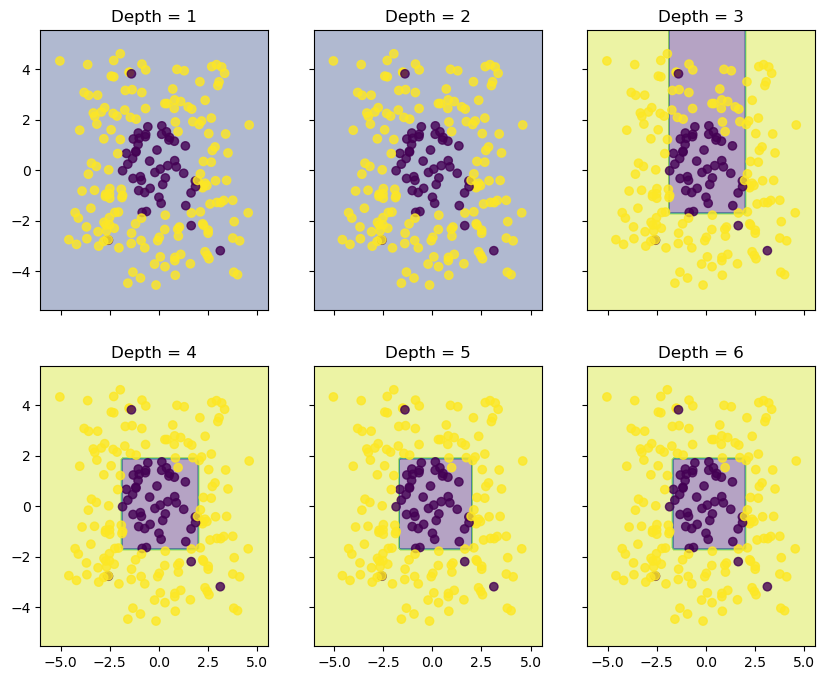
\includegraphics[width=10cm]{homework/homework_6/images/hw6_1.png}
           \item here is what sklearn's model produced with a min sample of 2 and max depth of 2 \\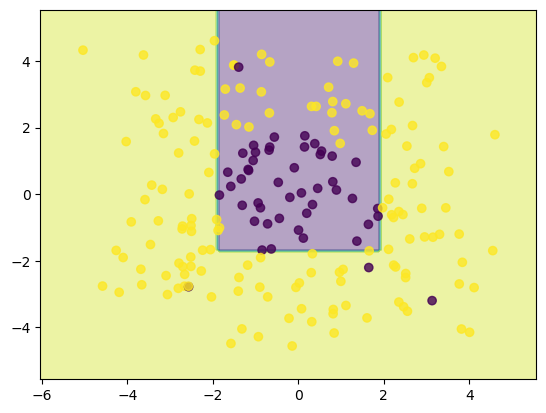
\includegraphics[width=10cm]{homework/homework_6/images/hw6_2.png}
           \item these plots are pretty similar so that is good
\end{itemize}
           


\item  Complete the function \texttt{mean\_absolute\_deviation\_around\_median}
(MAE). Use the code provided to fit the \texttt{Regression\_Tree} to
the krr dataset using both the MAE loss and median predictions. Include
the plots for the 6 fits.\\

 \begin{itemize}
           \color{blue}
               \item here is my MAE code \\
           \inputminted[firstline=298, lastline=311, breaklines=True]{python}{hw6.py}
           \item here is what my plots look like for min sample size of 3 and max depth 1,2,3,4,5,10 
           \\ 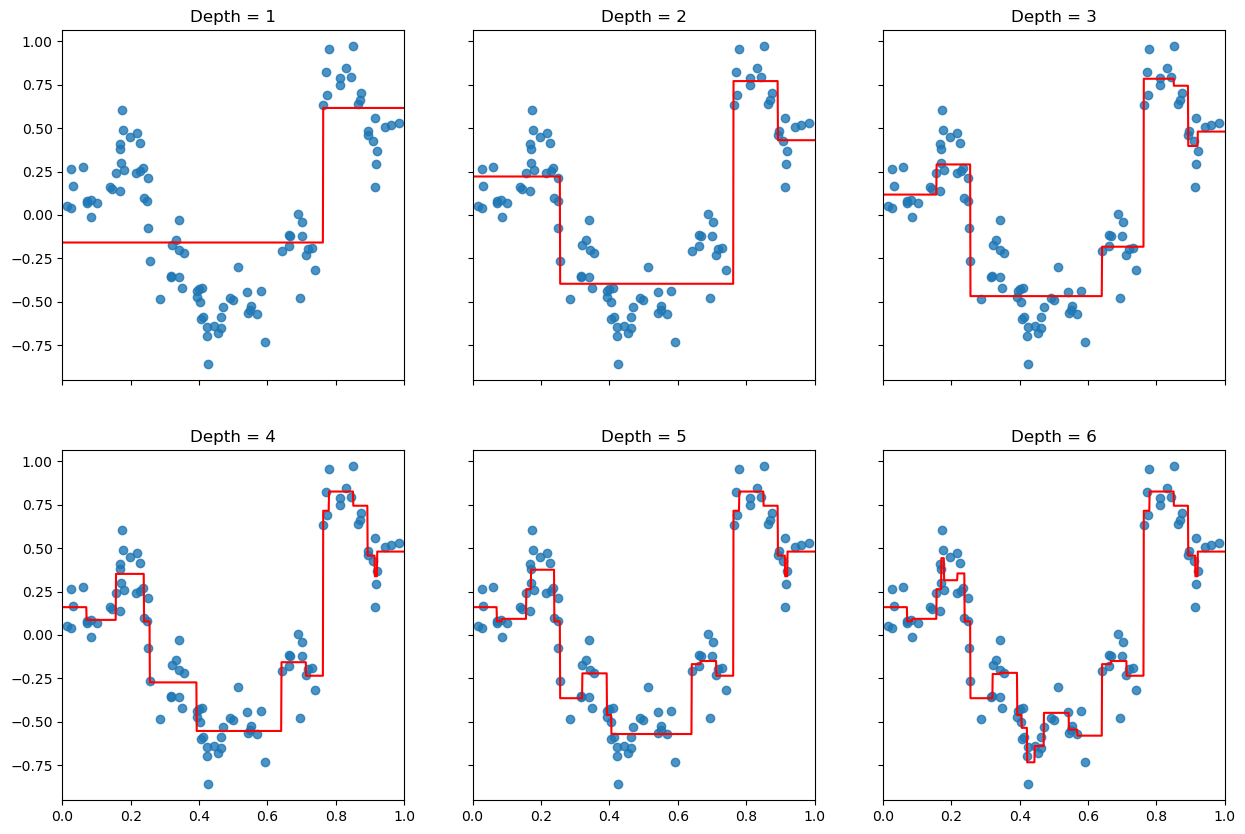
\includegraphics[width=15cm]{homework/homework_6/images/hw6_3.png
           }
\end{itemize}


\setcounter{saveenum}{\value{enumi}}
\end{enumerate}

\section{Ensembling}

Recall the general gradient boosting algorithm
% \footnote{Besides the lecture slides, you can find an accessible discussion
% of this approach in \url{http://www.saedsayad.com/docs/gbm2.pdf},
% in one of the original references \url{http://statweb.stanford.edu/~jhf/ftp/trebst.pdf},
% and in this review paper \url{http://web.stanford.edu/~hastie/Papers/buehlmann.pdf}. }
, for a given loss function $\ell$ and a hypothesis space $\cf$
of regression functions (i.e. functions mapping from the input space
to $\reals$): 
\begin{enumerate}
\setcounter{enumi}{\value{saveenum}}
\item[0:] Initialize $f_{0}(x)=0$. 
\item[1:] For $m=1$ to $M$:

\begin{enumerate}
\item Compute: 
\[
{\bf g}_{m}=\left( \frac{\partial}{\partial f_{m-1}(x_{j})}\sum_{i=1}^{n}\ell\left(y_{i},f_{m-1}(x_{i})\right)\right)_{j=1}^{n}
\]
\item Fit regression model to $-{\bf g}_{m}$: 
\[
h_{m}=\argmin_{h\in\cf}\sum_{i=1}^{n}\left(\left(-{\bf g}_{m}\right)_{i}-h(x_{i})\right)^{2}.
\]
\item Choose fixed step size $\nu_{m}=\nu\in(0,1]$, or take 
\[
\nu_{m}=\argmin_{\nu>0}\sum_{i=1}^{n}\ell\left(y_{i},f_{m-1}(x_{i})+\nu h_{m}(x_{i})\right).
\]
\item Take the step: 
\[
f_{m}(x)=f_{m-1}(x)+\nu_{m}h_{m}(x)
\]
\end{enumerate}
\item[3:] Return $f_{M}$. 
\end{enumerate}


This method goes by many names, including gradient boosting machines
(GBM), generalized boosting models (GBM), AnyBoost, and gradient boosted
regression trees (GBRT), among others. One of the nice aspects
of gradient boosting is that it can be applied to any problem with
a subdifferentiable loss function.


\nyuparagraph{Gradient Boosting Regression Implementation}
First we'll keep things simple and consider the standard regression setting with square loss. In this case the we have $\cy=\reals$, our
loss function is given by $
\ell(\hat{y},y)=1/2\left(\hat{y}-y\right)^{2}$,
and at the $m$'th round of gradient boosting, we
have
\[
h_{m}=\argmin_{h\in\cf}\sum_{i=1}^{n}\left[\left(y_{i}-f_{m-1}(x_{i})\right)-h(x_{i})\right]^{2}.
\]

\begin{enumerate}
\setcounter{enumi}{\value{saveenum}}
  
\item Complete the \texttt{gradient\_boosting} class. As the base regression
algorithm to compute the argmin, you should use sklearn's regression tree. You should use
the square loss for the tree splitting rule (\texttt{criterion} keyword argument) and use the default sklearn leaf prediction rule from the \texttt{predict} method \footnote{Examples of usage are given in the skeleton code to debug previous problems, and you can check the docs \url{https://scikit-learn.org/stable/modules/generated/sklearn.tree.DecisionTreeRegressor.html}}. We will also use a constant step size $\nu$.\\

 \begin{itemize}
           \color{blue}
               \item 
           \inputminted[firstline=440, lastline=492, breaklines=True]{python}{hw6.py}
\end{itemize}



\item Run the code provided to build gradient
boosting models on the regression data sets \texttt{krr-train.txt}, and
include the plots generated. For debugging you can use the sklearn implementation of \texttt{GradientBoostingRegressor}\footnote{\url{https://scikit-learn.org/stable/modules/generated/sklearn.ensemble.GradientBoostingRegressor.html}}.
\setcounter{saveenum}{\value{enumi}}\\


 \begin{itemize}
           \color{blue}
               \item 
           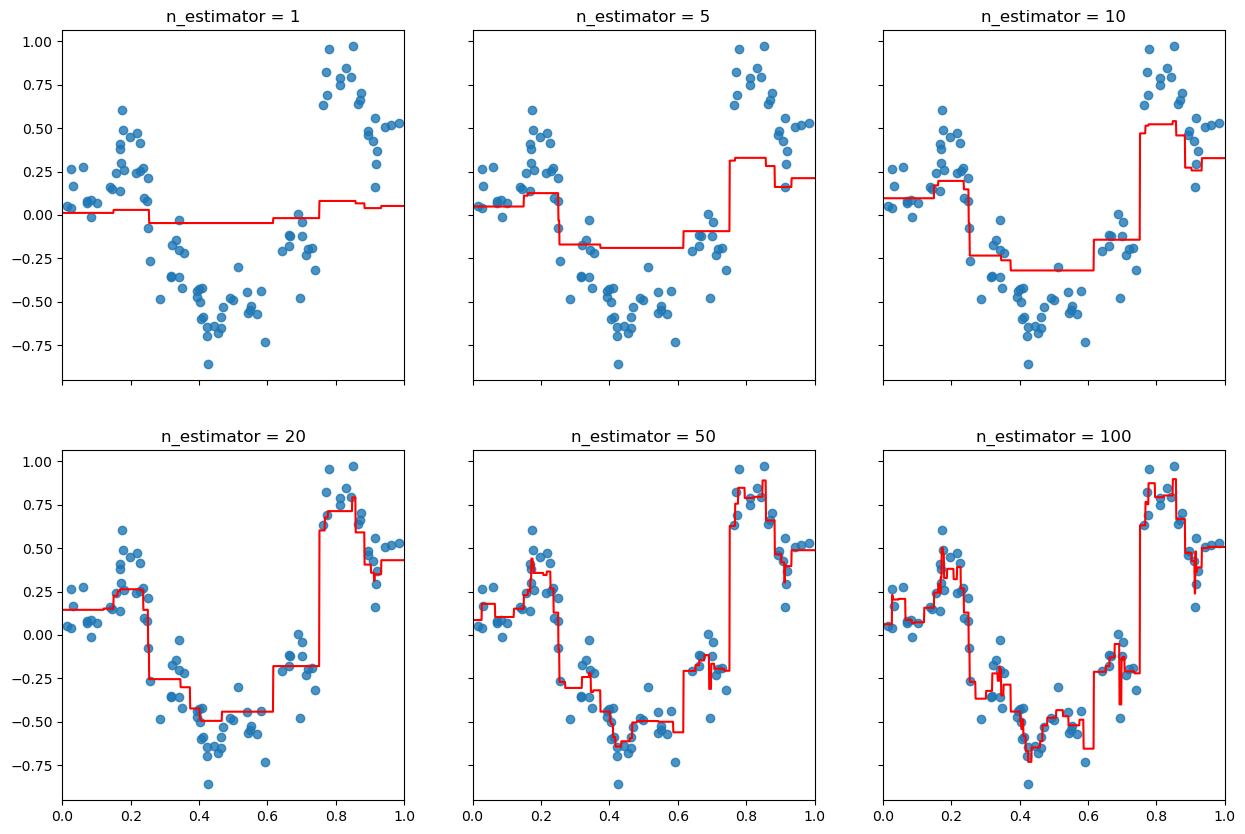
\includegraphics[width=15cm]{homework/homework_6/images/hw6_4.png}
\end{itemize}


\end{enumerate}

\nyuparagraph{Classification of images with Gradient Boosting}
In this problem we will consider the classification of MNIST, the dataset of handwritten digits images, with ensembles of trees. For simplicity, we only retain the `0' and '1' examples and perform binary classification.

First we'll derive a special case of the general gradient
boosting framework: BinomialBoost. 
Let's consider the classification framework, where $\cy=\left\{ -1,1\right\} $.
In lecture, we noted that AdaBoost corresponds to forward stagewise
additive modeling with the exponential loss, and that the exponential
loss is not very robust to outliers (i.e. outliers can have a large
effect on the final prediction function). Instead, let's consider
the logistic loss 
\[
\ell(m)=\ln\left(1+e^{-m}\right),
\]
where $m=yf(x)$ is the margin.

\begin{enumerate}
  \setcounter{enumi}{\value{saveenum}}
  
\item Give the expression of the negative gradient step direction, or pseudo residual, $-{\bf g}_{m}$ for the logistic loss as a function of the prediction function $f_{m-1}$ at the previous iteration and the dataset points $\{(x_i, y_i)\}_{i=1}^n$. What is the dimension of $g_{m}$?\\


\begin{itemize}
    \color{blue}
    \item we can write $\ell(x_i,y_i)=ln(1+e^{-y_if(x_i)})$
    \item further the psuedo resisted for the ith example is given the negative partial derivative of the loss with respect to our current prediction function (that is the function we have learned up to step $m-1 $   $g_i=-\frac{\partial \ell(y_i, f_{m-1}(x_i))}{\partial f_{m-1}(x_i)}=-\frac{\partial ln(1+e^{-y_if_{m-1}(x_i)})}{\partial f_{m-1}(x_i)}=\frac{y_ie^{-y_if_{m-1}(x_i)}}{1+e^{-y_if_{m-1}(x_i)}}=\frac{y_i}{1+e^{y_if_{m-1}(x_i)}}$
    \item there are n total tuples of the form $(x_i,y_i)$ in our dataset thus $g=$ \begin{pmatrix}\frac{\partial \ell(y_i, f_{m-1}(x_1))}{\partial f_{m-1}(x_1)}\\\cdots\\\frac{\partial \ell(y_i, f_{m-1}(x_1))}{\partial f(x_n)}
    \end{pmatrix}$ \in \mathbb{R}^{n}$
\end{itemize}

\item Write an expression for $h_{m}$ as an argmin over functions $h$ in $\cf$.\\

\begin{itemize}
    \color{blue}
    \item given our base hypothesis space $\mathcal{H}$
    \item our value for $h_m$ will be given as $$h_m=argmin_{h\in \mathcal{H}}\Sigma_{i=1}^{n}[-g_i-h(x_i)]^2=argmin_{h\in \mathcal{H}}\Sigma_{i=1}^{n}[(\frac{y_i}{1+e^{y_if_{m-1}(x_i)}})-h(x_i)]^2$$
\end{itemize}


  
\item Load the MNIST dataset using the helper preprocessing function in the skeleton code.Using the scikit learn implementation of \texttt{GradientBoostingClassifier}, with the logistic loss (\texttt{loss=`deviance'}) and trees of maximum depth 3, fit the data with 2, 5, 10, 100 and 200 iterations (estimators). Plot the train and test accurary as a function of the number of estimators.\\

 \begin{itemize}
           \color{blue}
               \item 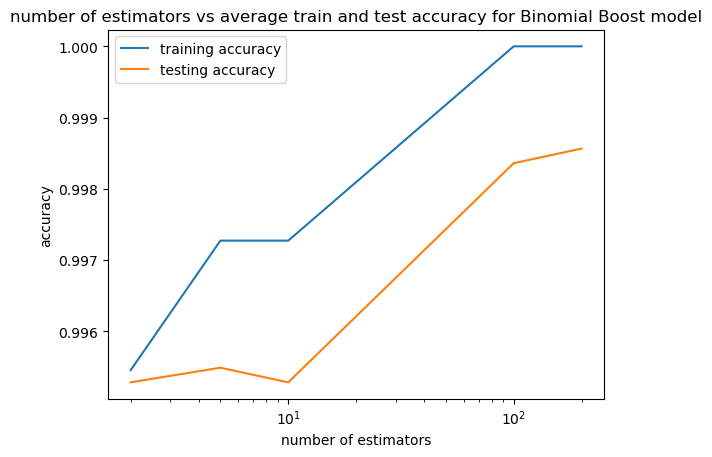
\includegraphics[width=15cm]{homework/homework_6/images/hw6_5.png}
\end{itemize}

\setcounter{saveenum}{\value{enumi}}
\end{enumerate}

\nyuparagraph{Classification of images with Random Forests (Optional)}
\begin{enumerate}
  \setcounter{enumi}{\value{saveenum}}
\item Another type of ensembling method we discussed in class are random forests. Explain in your own words the construction principle of random forests.\\


\begin{itemize}
    \color{blue}
    \item single trees tend to overfit the data they are trained on and thus have high variance. 
    \item they however are very simple, inheritable and can fit non-linear relationships and thus are ideal for ensemble models 
    \item both bagging trees and random forests, aim to build parallel ensemble models, that is they build all their models at the same time (as opposed to sequential models) 
    \item Bagging does this by training many independent smaller trees on boostrapped samples of the data, which is theoretically great, however the assumption of Independence between the trees is violated by the boostrapping process. this means that if we are trying to fit a large number of trees with the bagging procedure our trees will become high correlated, and the goal of averaging across them to reduce variance is lost 
    \item random forest try to avoid the dependence between tries by modifying each of the inner trees training process. 
    \item this is done by allowing each tree to only split on some random subset of the total features of our dataset. this prevents a case where all of trees would be completely determined by a small number of highly predictive features. 
\end{itemize}

\item Using the scikit learn implementation of \texttt{RandomForestClassifier}\footnote{\url{https://scikit-learn.org/stable/modules/generated/sklearn.ensemble.RandomForestClassifier.html\#sklearn.ensemble.RandomForestClassifier}},
with the entropy loss (\texttt{criterion=`entropy'}) and trees of maximum depth 3, fit the preprocessed binary MNIST dataset with 2, 5, 10, 50, 100 and 200 estimators.\\

 \begin{itemize}
           \color{blue}
               \item 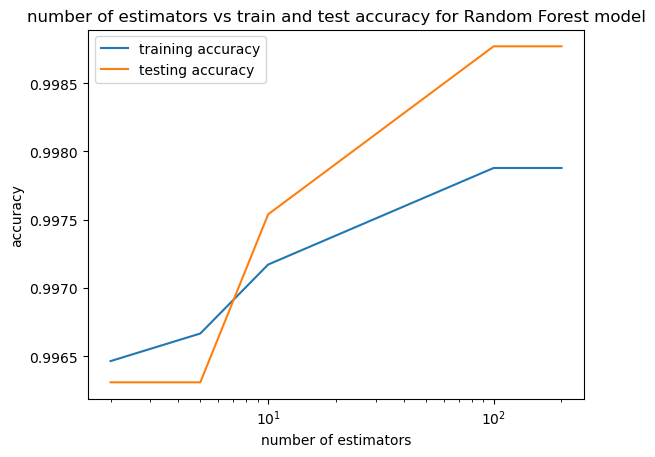
\includegraphics[width=15cm]{homework/homework_6/images/hw6_6.png}
\end{itemize}



\item What general remark can you make on overfitting for Random Forests and Gradient Boosted Trees? Which method achieves the best train accuracy overall? Is this result expected? 
Can you think of a practical disadvantage of the best performing method? How do the algorithms compare in term of test accuracy? \\
\begin{itemize}
    \color{blue}
    \item both random forest and Gradient boosted classification models in general tend to overfit. It does not appear that this was the case in this example, this is likely due to the fact that we are only using max depth =3 for each learner so all independent learners are fairly week. this is evidenced as in both cases the accuracy of model on the training data and test data seems to be increasing in the number of estimators. where as we would expect if the models were over fitting the testing accuracy to start falling at some point 
    \item the Gradient boosted classification model has a very slight  advantage in terms train accuracy with an average accuracy of 1 compared to the best training accuracy of the random forest model being 0.9978.
    \item yes this is expected as gradient boosted classification is a sequential, which fits each week learner to correct the error of the last which will naturally fit tend to fit the training data pretty closely compared to random forests which are a parallel ensemble model which fit n weak learners all at once on different subsets of the datas features, so it makes sense gradient boosted classification would do better. 
    \item a disadvantage of gradient boosted classifiers is they take much longer to train for only a slight increase in training accuracy, and as it is a sequential model the gradient boosted classifier could overfit the data.  
    \item the Gradient boosting classifier having a higher test accuracy of 0.9985 and the random forest having a test accuracy of 0.9987 so we slightly better test accuracy on the random forest model
    \item this is expected because both models have similar train accuracy, and the random forest is parallel so we would expect it to overfit less. 
\end{itemize}


\setcounter{saveenum}{\value{enumi}}
\end{enumerate}

\end{document}
